\section{Scope}
This section lists World, Shared and Machine Phenomena in order to identify in a precise way the environment in which the application operates. \\
\textbf{World Phenomena}
\begin{itemize}
	\item $W_1$ : Customers arrive to the supermarket.
	\item $W_2$ : Customers enter the supermarket.
	\item $W_3$ : The store managers hand out tickets on spot.
\end{itemize}
\textbf{Shared Phenomena}\\
\textit{Controlled by the World and observed by the Machine:}
\begin{itemize}
	\item $S_1$ : Customers make line-up requests.
	\item $S_2$ : Customers indicate with which mean of transport they intend to go the supermarket.
	\item $S_3$ : Customers scan their QR codes.
	\item $S_4$ : Customers book visits.
	\item $S_5$ : Customers input the duration of the visits.
	\item $S_6$ : Customers input items to buy or their categories.
\end{itemize}
\textit{Controlled by the Machine and observed by the World:}
\begin{itemize}
	\item $S_7$ : The system shows customers their waiting time.
	\item $S_8$ : The system notifies customers when they have to start.
	\item $S_9$ : The system generates tickets for the for customers who don't have the required technology.
	\item $S_{10}$ : The system sends QR codes to customers.
	\item $S_{11}$ : The system retrieves the GPS position of the customer.
	\item $S_{12}$ : The system increases entrances monitoring the affluence of the departments.
\end{itemize}
\textbf{Machine Phenomena}
\begin{itemize}
	\item $M_1$ : The system manages real-time queue.
	\item $M_2$ : The system calculate the waiting time for the single customer.
	\item $M_3$ : The system generates QR codes.
	\item $M_4$ : The system optimizes the planning of visits.
	\item $M_5$ : The system infer the visit time of long-term users. 
\end{itemize} 

\begin{figure}[H] 
\centerline{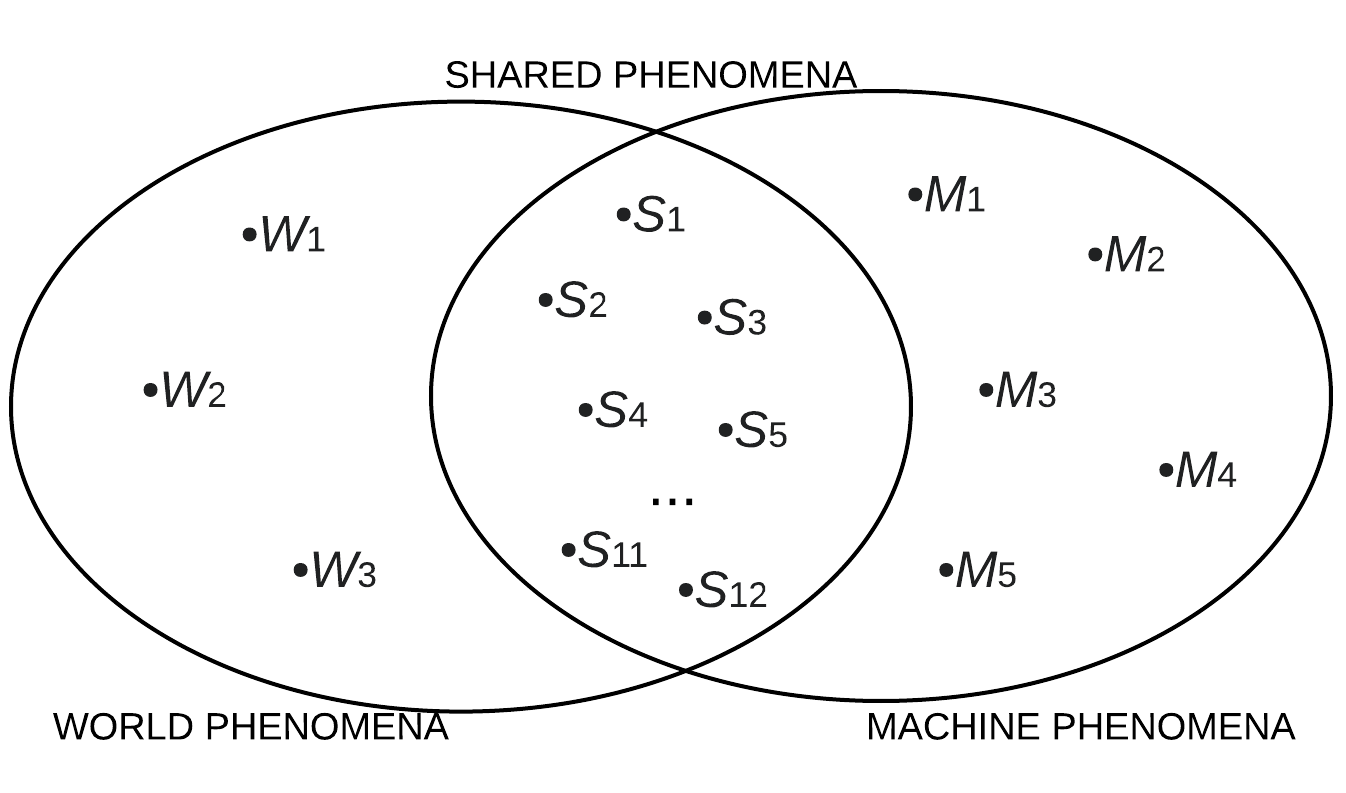
\includegraphics[scale=0.5]{WSMPhenomena}}
\caption{World, Shared and Machine Phenomena}
\end{figure}


